%% Use \documentclass[print]{dissertation} to export the document
\documentclass[]{dissertation}

\graphicspath{
  {images/}
  {thesis_introduction/}
  {babette_article/article/}
  {pirouette_article/}
  {razzo_article/}
  {thesis_synthesis/}
}

\usepackage{authblk}

\usepackage{booktabs}
\usepackage{siunitx} % handle units with proper spacing
\usepackage[final]{pdfpages} % add pdf pages
\usepackage{gensymb} % \degree symbol
\usepackage{afterpage} %page selection and control 
\usepackage{adjustbox} % Limit table
\usepackage{colortbl} % colors in tables.
\usepackage{rotating} % table rotation
\usepackage{microtype} % improves reading
\usepackage{textcomp} %fix apostrophes
\usepackage{textgreek}

\usepackage{listings}
\usepackage{hyperref}
\usepackage{todonotes}
\usepackage{verbatim}
\usepackage{pgf}
\usepackage{bm}

% Style of listings
% From http://r.789695.n4.nabble.com/How-to-nicely-display-R-code-with-the-LaTeX-package-listings-tp4648110.html
\usepackage{fancyvrb} 
\definecolor{codegreen}{rgb}{0,0.6,0}
\definecolor{codegray}{rgb}{0.5,0.5,0.5}
\definecolor{codepurple}{rgb}{0.58,0,0.82}
\definecolor{backcolor}{rgb}{0.95,0.95,0.92}
\lstdefinestyle{mystyle}{
  language=R,% set programming language
  basicstyle=\ttfamily\small,% basic font style
  commentstyle=\color{gray},% comment style
  % numbers=left,% display line numbers on the left side
  numberstyle=\scriptsize,% use small line numbers
  numbersep=10pt,% space between line numbers and code
  tabsize=2,% sizes of tabs
  showstringspaces=false,% do not replace spaces in strings by a certain character
  captionpos=b,% positioning of the caption below
  breaklines=true,% automatic line breaking
  escapeinside={(*}{*)},% escaping to LaTeX
  fancyvrb=true,% verbatim code is typset by listings
  extendedchars=false,% prohibit extended chars (chars of codes 128--255)
  alsoletter={.<-},% becomes a letter
  alsoother={$},% becomes other
  otherkeywords={!=, ~, $, \&, \%/\%, \%*\%, \%\%, <-, <<-, /},% other keywords
  deletekeywords={c}% remove keywords 
}
\lstset{style=mystyle}

% Use 'It was found that A is B (Name 1234)' style
\setcitestyle{authoryear,open={},close={}}

% To put figures 'Here'
\usepackage{float}

% subfigure
\usepackage{subfig}
\usepackage{graphicx}

% Need this, but needs to be installed
% \usepackage{multibib}

% TikZ drawing
\usetikzlibrary{arrows,automata}
\usetikzlibrary{calc}
\usetikzlibrary{arrows.meta}

% break long URLs
\usepackage{hyperref}
\def\UrlBreaks{\do\/\do-}

%%%%%%%%%%%%%%%%%%%%%%%%%%%%%%%%%%%%%%%%%%%%%%%%%%%%%%%%%%%%%%%%%%%%%%%%%%%%%%%%
% Feedback commands
%%%%%%%%%%%%%%%%%%%%%%%%%%%%%%%%%%%%%%%%%%%%%%%%%%%%%%%%%%%%%%%%%%%%%%%%%%%%%%%%
\newcommand{\giovanni}[1]{\textcolor{blue}{\textbf{[GL: #1]}}}
\newcommand{\richel}[1]{\textcolor{orange}{\textbf{[RB: #1]}}}
\newcommand{\rampal}[1]{\textcolor{green}{\textbf{[RSE: #1]}}}
\newcommand{\gio}[1]{\textcolor{blue}{\textbf{[GL: #1]}}}
%%%%%%%%%%%%%%%%%%%%%%%%%%%%%%%%%%%%%%%%%%%%%%%%%%%%%%%%%%%%%%%%%%%%%%%%%%%%%%%%

\raggedbottom % remove unwanted spaces between paragraphs
%%%% List of common used terms

\begin{document}

%% Specify the title and author of the thesis. This information will be used on
%% the title page (in title/title.tex) and in the metadata of the final PDF.
\title{The error in trees without birds}
\author{Rich\`el}{Bilderbeek}

%% Use Roman numerals for the page numbers of the title pages and table of
%% contents.
\frontmatter

\begin{titlepage}
%	\includepdf[pages=-]{front_cover.pdf}

% The easiest way to cope with RuG font requirements is just use your favorite text editor (word, libre) and export that to PDF. Remember to set your page to B5! There's a .doc file attached.
	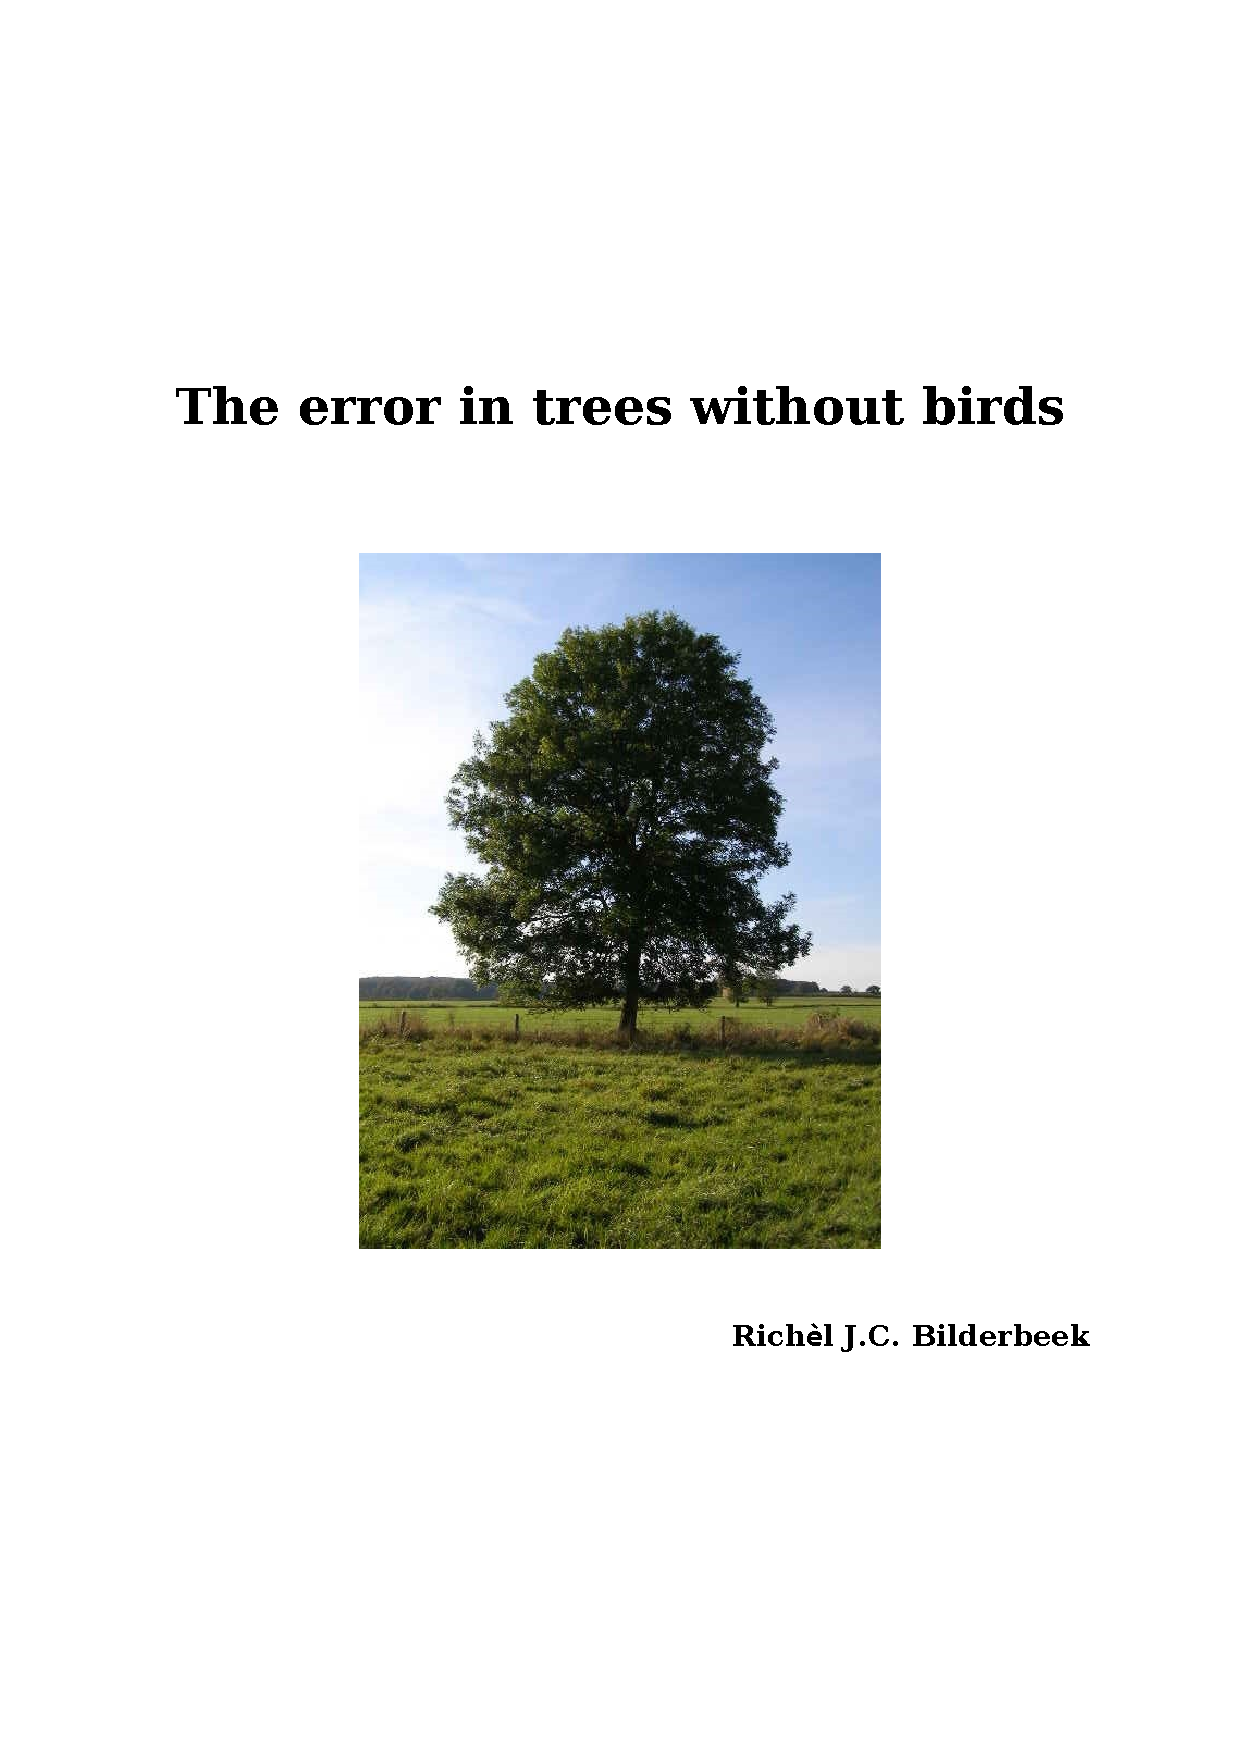
\includepdf[pages=-]{title/firstpage.pdf}
	
	
	%%%%%%%%%%%%%%%%%%%%%%%%%%%%% Book information page %%%%%%%%%%%%%%%%%%%%%%%%%%%%%%%%%%%%%
	
	\newpage \thispagestyle{empty}
	\vspace*{3.9cm}%{4.7cm} was 5.7, save 2 for FSC logo
	
	
	\begin{figure}[!h]
		
\includegraphics[width=\textwidth]{images/frontmatter/zernike.pdf}
	\end{figure}
	
	\vfill
	\begin{figure}[!h]
		
\includegraphics[width=\textwidth]{images/frontmatter/all-logos.pdf}
	\end{figure}
	\noindent
	{\small 
		Zernike Institute PhD thesis series 2016-12 \\
		ISSN:   1570-1530\\
		ISBN:	978-90-367-8806-9 \\
		ISBN:   978-90-367-8805-2 (electronic version) \\
		\\
		The work described in this thesis was performed in the research group Single Molecule Biophysics of the Zernike Institute for Advanced Materials at the University of Groningen, the Netherlands. \\
		\\
		Cover design: Victor E. A. Caldas\\
		Cover image: Super-resolution image reconstruction o \textit{E. coli} cells. Membrane marker (red) is LacY-eYFP and blue is UmuC-mKate2.
		\\
			%	An electronic version of this dissertation is available at: \\
	%	\url{http://MYTHESIS.COM}
		Printed by: GVO drukkers \& vormgevers B.V. \\
		} 	
	
	
	\clearpage
	
	
\includepdf[pages=-]{title/titlepage.pdf}
	
\end{titlepage}


\tableofcontents

%% Use Arabic numerals for the page numbers of the chapters.
\mainmatter

%% Turn on thumb indices.
\thumbtrue



%%%%%%%%%%%%%%%%%%%%%%%%%%%%%%%%%%%%%%%%%%%%%%%%%%%%%%%%%%%%%%%%%%%%%%%%%%%%%%%%
% Introduction
%%%%%%%%%%%%%%%%%%%%%%%%%%%%%%%%%%%%%%%%%%%%%%%%%%%%%%%%%%%%%%%%%%%%%%%%%%%%%%%%
\references{thesis_introduction/introduction}
\section{First section of introduction}

wgfewerqg

\section{Second section of introduction}

ergqerg
\references{thesis_introduction/introduction}
\input{thesis_introduction/introduction_photo_attribution}

\iffalse

  %%%%%%%%%%%%%%%%%%%%%%%%%%%%%%%%%%%%%%%%%%%%%%%%%%%%%%%%%%%%%%%%%%%%%%%%%%%%%%%%
  % babette
  %%%%%%%%%%%%%%%%%%%%%%%%%%%%%%%%%%%%%%%%%%%%%%%%%%%%%%%%%%%%%%%%%%%%%%%%%%%%%%%%
  \chapter{babette: BEAUti 2, BEAST2 and Tracer for R}
  \label{chapter_babette}
  Rich\`el J.C. Bilderbeek, Rampal S. Etienne
  \newpage
  \include{babette_article/article/babette_content}
  \references{babette_article/article/babette_article}
  \include{babette_article/article/babette_figure_1}

  %%%%%%%%%%%%%%%%%%%%%%%%%%%%%%%%%%%%%%%%%%%%%%%%%%%%%%%%%%%%%%%%%%%%%%%%%%%%%%%%
  % pirouette
  %%%%%%%%%%%%%%%%%%%%%%%%%%%%%%%%%%%%%%%%%%%%%%%%%%%%%%%%%%%%%%%%%%%%%%%%%%%%%%%%
  \chapter{pirouette}
  \label{chapter_pirouette}
  Rich\`el J.C. Bilderbeek, Giovanni Laudanno, Rampal S. Etienne
  \newpage
  \references{pirouette_article/article}
  \include{pirouette_article/content}
  \include{pirouette_article/supplement}

  %%%%%%%%%%%%%%%%%%%%%%%%%%%%%%%%%%%%%%%%%%%%%%%%%%%%%%%%%%%%%%%%%%%%%%%%%%%%%%%%
  % razzo
  %%%%%%%%%%%%%%%%%%%%%%%%%%%%%%%%%%%%%%%%%%%%%%%%%%%%%%%%%%%%%%%%%%%%%%%%%%%%%%%%
  \chapter{razzo}
  \label{chapter_razzo}
  Giovanni Laudanno, Rich\`el J.C. Bilderbeek, Rampal S. Etienne
  \newpage
  \input{razzo_article/razzo-abstract.tex}
  \input{razzo_article/razzo-introduction.tex}
  \input{razzo_article/razzo-methods.tex}
  razzo_article/tab_simparameters.tex
  \input{razzo_article/razzo-results.tex}
  \input{razzo_article/fig_results.tex}
  \input{razzo_article/razzo-discussion.tex}
  \input{razzo_article/razzo-supplement.tex}


\fi

%%%%%%%%%%%%%%%%%%%%%%%%%%%%%%%%%%%%%%%%%%%%%%%%%%%%%%%%%%%%%%%%%%%%%%%%%%%%%%%%
% Synthesis
%%%%%%%%%%%%%%%%%%%%%%%%%%%%%%%%%%%%%%%%%%%%%%%%%%%%%%%%%%%%%%%%%%%%%%%%%%%%%%%%
\references{thesis_synthesis/synthesis}
\include{thesis_synthesis/synthesis}

%% Use letters for the chapter numbers of the appendices.
\appendix

%% Turn off thumb indices for unnumbered chapters.
\thumbfalse

%%%%%%%%%%%%%%%%%%%%%%%%%%%%%%%%%%%%%%%%%%%%%%%%%%%%%%%%%%%%%%%%%%%%%%%%%%%%%%%%
% CV
%%%%%%%%%%%%%%%%%%%%%%%%%%%%%%%%%%%%%%%%%%%%%%%%%%%%%%%%%%%%%%%%%%%%%%%%%%%%%%%%
\chapter*{Curriculum Vit\ae}
\addcontentsline{toc}{chapter}{Curriculum Vit\ae}
\setheader{Curriculum Vit\ae}

%% Print the full name of the author.
\makeatletter
%\authors{\@firstname\ {\titleshape\@lastname}}
\authors{Rich\`el J.C. Bilderbeek}
\makeatother

\noindent
\begin{tabular}{p{4\parindent}l}
    02-09-1980 & Born in Milsbeek, The Netherlands.
\end{tabular}

\section*{Education}

\begin{tabular}{p{4\parindent}l}
    1999--2005 & Undergraduate in Biology \\
    & Rijksuniversiteit Groningen \\
    \\
    2007--2008 & Undergraduate in Pre-higher Education in Biology \\
    & Rijksuniversiteit Groningen \\
    \\
    2011--2014 & Undergraduate in Mechatronics \\
    & Alfa College Groningen \\
    \\
    2014-2019 & PhD.\ Theoretical Biology  \\
    & Rijksuniversiteit Groningen \\
    &
    %% The width of the second column is the width of the page, minus the width
    %% of the first column (4\parindent) minus four times the separation between
    %% the start of the column and its contents.
    \begin{minipage}{\textwidth-4\parindent-4\tabcolsep}
        %% We divide the minipage 20/80.
        \begin{tabular}{@{}p{0.2\linewidth}@{}p{0.8\linewidth-\tabcolsep}}
            \textit{Thesis:} & The error in trees without birds \\
            \textit{Promotor:} & Prof.\ dr.\ R.\ S.\ Etienne
        \end{tabular}
    \end{minipage}
\end{tabular}

\section*{Work experience}

\begin{tabular}{p{4\parindent}l}
    2004--2018 & Software developer, many projects \\
    \\
    2008--2010 & Secondary school teacher, in stagecraft, biology, physics, chemistry \\
               & VMBO 't Venster Arnhem \\
\end{tabular}

\section*{Volunteering}

\begin{tabular}{p{4\parindent}l}
    2014--now & Coordinator of courses in programming and digital electronics \\
              & Stichting De Jonge Onderzoekers Groningen \\
    \\
%    2016--now & Arcwelder \\
%              & Corsowijk de Korenbloem Eelde \\
%    \\
    2000--2012 & Light and sound technician \\
              & Prinsentheater Groningen \\
\end{tabular}


\end{document}

